\chapter{Analisi dinamiche}
In questa sezione vengono presentati gli strumenti utilizzati per effettuare le scansioni dinamiche. I risultati verranno aggregati e commentati insieme a quelli delle analisi statiche nella sezione $3$.

%----------------------------------------------------%
%-------------------- DROZER ------------------------%
%----------------------------------------------------%

\section{Drozer}

\begin{figure}[h]
	\centering 
	
\includegraphics[width=.45\textwidth]{/drozer/logo} 
	\caption{Drozer}
	\label{fig:drozer}
\end{figure}

Drozer\cite{Drozer} è un software open source, rilasciato e mantenuto da MWR InfoSecurity e licenziato tramite BSD. Drozer permette di assumere il ruolo di un'applicazione Android installata all'interno del dispositivo e di interagire con le altre applicazioni presenti.

Attraverso l'utilizzo di un agent Drozer si può fare tutto quello che un'applicazione installata nel dispositivo può fare (interagire con la Dalvik VM, utilizzare il meccanismo di \ac{IPC} o interagire col sistema operativo sottostante). L'agent fungerà da interfaccia di amministrazione remota e rappresenterà un'applicazione non privilegiata. L'agent richiede un solo permesso al sistema operativo: il permesso INTERNET, necessario per aprire la socket e connettersi con la console o il server. 

Drozer è in grado di costruire contenuti malevoli per eseguire exploit su vulnerabilità note e di caricarle sull'agent.

A seconda dei permessi concessi all'applicazione vulnerabile, Drozer è in grado di installare un agent completo, iniettare un agent limitato dentro al processo relativo all'applicazione o generare una reverse shell.

La particolarità di Drozer sta nell'assoluta indipendenza da strumenti come ADB o \ac{AAPT} che richiederebbero una connessione USB al dispositivo. Essa avviene infatti esclusivamente tramite rete (di default sulla porta TCP:$31415$).

\subsection{Utilizzo}
Drozer è in grado di eseguire svariate azioni:
\begin{itemize}
	\item \textbf{Ricavare le informazioni sui pacchetti installati nel dispositivo}. Il comando in figura \ref{fig:drozerList} dispone di numerosi filtri come ad esempio quello sui permessi richiesti. Nella figura, sono state listate le applicazioni che richiedono il permesso RECORD AUDIO tra le quali compare anche l'applicazione che stiamo testando.
	\begin{figure}[h]
		\centering 
		\fbox{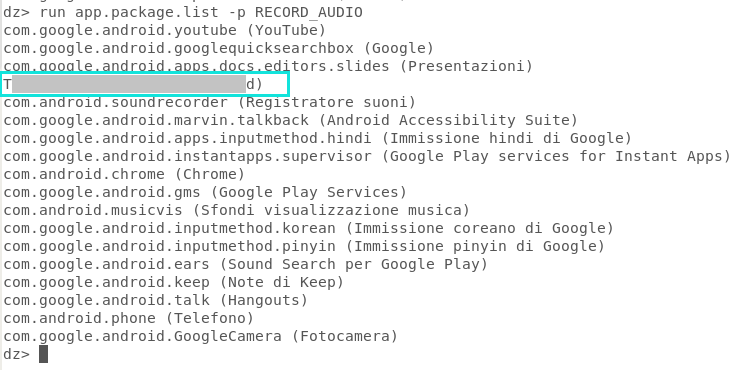
\includegraphics[width=.9\textwidth]{/drozer/drozerListBN}} 
		\caption{Elenco di applicazioni che richiedono il permesso RECORD AUDIO.}
		\label{fig:drozerList}
	\end{figure}

	\item \textbf{Ricavare le informazioni su un singolo pacchetto}. Il comando utilizzato nella figura \ref{fig:appInfo} permette di ricavare le informazioni di base di qualsiasi applicazione installata nel dispositivo. In questo caso sono le informazioni riguardanti l'applicazione testata.
	\begin{figure}[h]
		\centering 
		\fbox{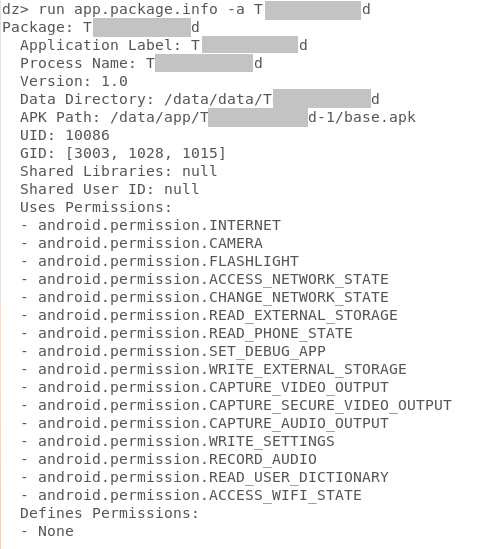
\includegraphics[width=.6\textwidth]{/drozer/appInfoBN}} 
		\caption{Informazioni sull'applicazione testata.}
		\label{fig:appInfo}
	\end{figure}

	\item \textbf{Identificare la possibile superficie d'attacco di un'applicazione}. Il comando in figura \ref{fig:attackSurface} cerca componenti esportati (activities, broadcast receivers e content providers) o per i quali è attivata la modalità di \emph{debug}. Lanciato sull'applicazione sotto test, si può notare come l'unico componente esportato sia l'activity principale e che la modalità di debug non sia attiva su alcun componente.
	\begin{figure}[h]
		\centering 
		\fbox{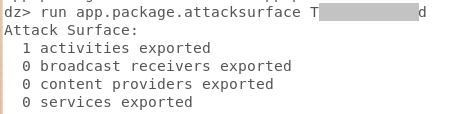
\includegraphics[width=.7\textwidth]{/drozer/attackSurfaceBN}} 
		\caption{Analisi della superficie d'attacco.}
		\label{fig:attackSurface}
	\end{figure}

	\item \textbf{Elencare e lanciare tutte le activities esportate da un'applicazione}. I due comandi riportati in figura \ref{fig:activities} rispettivamente, elencano tutte le activities esportate da un'applicazione e le eseguono. Nel nostro caso, l'unica activity esportata è quella che carica la schermata principale e la sua esecuzione fa semplicemente partire l'applicazione. 
	\begin{figure}[h]
		\centering 
		\fbox{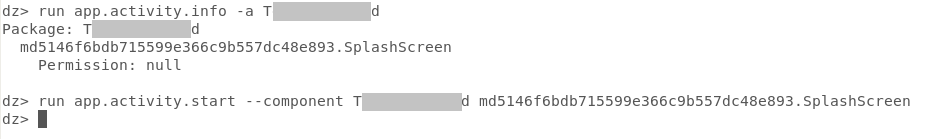
\includegraphics[width=.8\textwidth]{/drozer/activityBN}} 
		\caption{Elenco delle attività ed esecuzione.}
		\label{fig:activities}
	\end{figure}

	\item \textbf{Interagire con i \emph{content providers}}. È possibile listare ed interagire con i content providers esportati dalle applicazioni. Drozer fornisce anche uno scanner che mette insieme diverse tecniche per trovare paths ed inferire liste di possibili URI accessibili. È in grado anche di effettuare SQL injection se vengono rilevati database SQLite. Nell'applicazione testata non sono presenti content providers e il risultato è vuoto (figura \ref{fig:provider}).
	\begin{figure}[h]
		\centering 
		\fbox{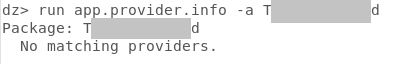
\includegraphics[width=.7\textwidth]{/drozer/providerBN}} 
		\caption{Elenco dei provider esportati.}
		\label{fig:provider}
	\end{figure}

	\item \textbf{Interagire con i servizi}. Come per i content providers, è possibile interagire con i servizi esportati. Anche in questo caso però, l'applicazione non presenta servizi esportati e quindi il risultato è vuoto (figura \ref{fig:services}).
	\begin{figure}[h]
		\centering 
		\fbox{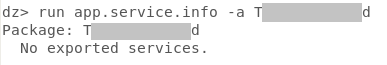
\includegraphics[width=.7\textwidth]{/drozer/servicesBN}} 
		\caption{Elenco dei servizi esportati.}
		\label{fig:services}
	\end{figure}

	\item \textbf{Opzioni avanzate}. Ulteriori comandi permettono di eseguire operazioni avanzate. \emph{shell.start} ad esempio, fa partire una shell linux interattiva sul dispositivo mentre \emph{tools.setup.busybox} vi installa \emph{busybox}.
\end{itemize}

%----------------------------------------------------%
%-------------------- SCROUNGER ---------------------%
%----------------------------------------------------%

\section{Scrounger}
\begin{figure}[h]
	\centering 
	
\includegraphics[width=.7\textwidth]{/scrounger/bannerBN} 
	\caption{Scrounger.}
	\label{fig:scrounger}
\end{figure}
Scrounger\cite{Scrounger} è uno strumento multipiattaforma (Android e iOS) dall'utilizzo simile a \emph{Metasploit}. Si presenta infatti con una console dalla quale è possibile eseguire dei comandi ed è composto da svariati moduli che permettono di automatizzare molte azioni necessarie nell'assessment di sicurezza di una applicazione mobile. È anche possibile scrivere i propri moduli ed eseguirli nella console principale del programma.

\subsection{Utilizzo}
Quando viene lanciato, Scrounger si presenta con una console molto simile a Metasploit dalla quale possiamo, ad esempio, elencare tutti i possibili moduli che riguardano Android (figura \ref{fig:lista}).
\begin{figure}[h]
	\centering 
	\fbox{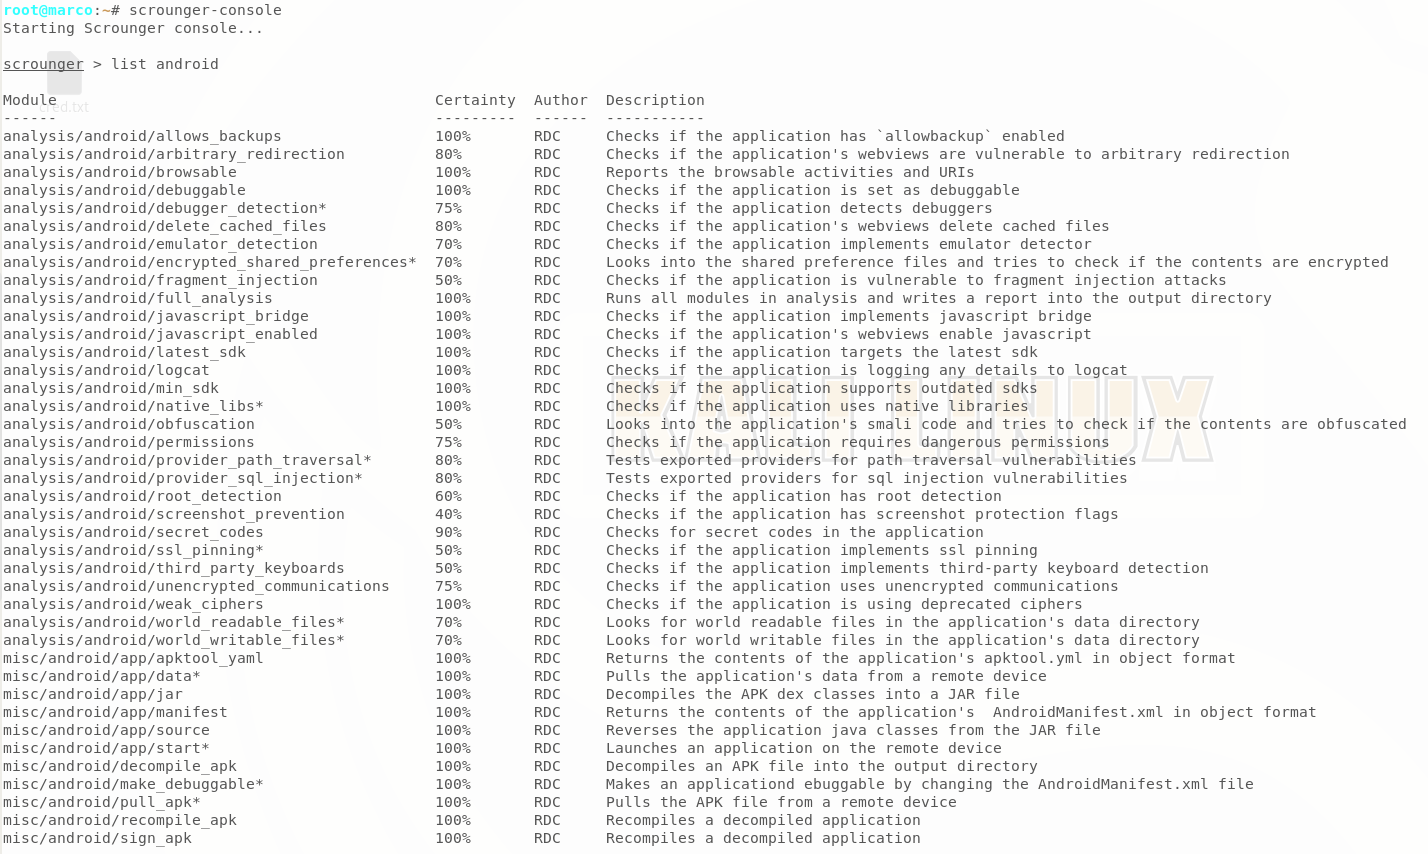
\includegraphics[width=.9\textwidth]{/scrounger/listaBN}}
	\caption{Moduli Android.}
	\label{fig:lista}
\end{figure}

Se volessimo verificare la possibilità di effettuare backup della nostra applicazione, potremmo utilizzare il modulo \emph{analysys/android/allow-backup} (figura \ref{fig:example}).
\begin{figure}[h]
	\centering 
	\fbox{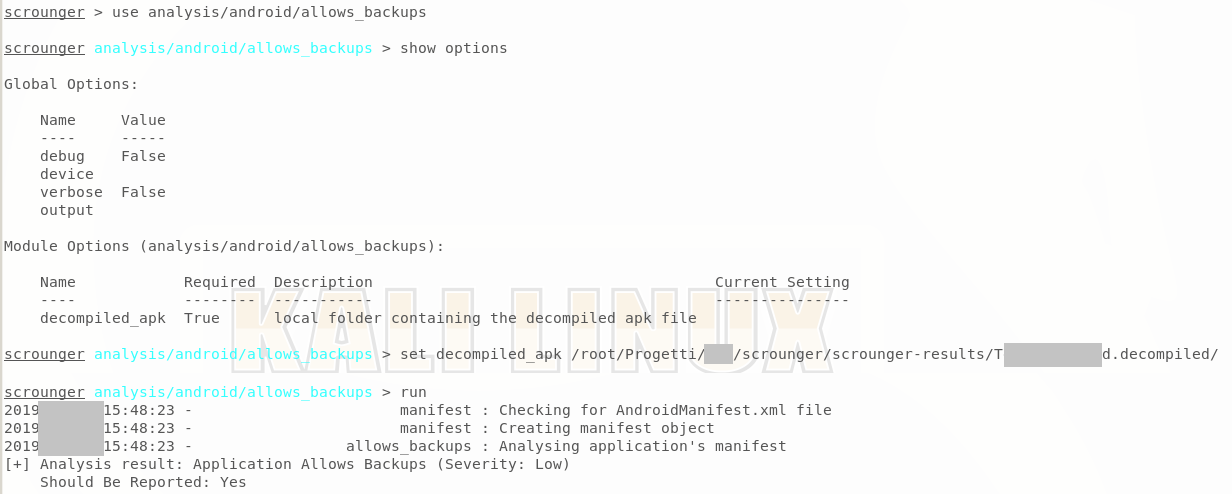
\includegraphics[width=.85\textwidth]{/scrounger/exampleCensBN}} 
	\caption{Un modulo di Scrounger.}
	\label{fig:example}
\end{figure}

Tramite il modulo \emph{android$/$full-analysys} è possibile eseguire automaticamente tutti i moduli inerenti ad Android. Per utilizzarlo è necessario collegare un device (meglio se con disponibilità dei privilegi di root) tramite adb che verrà utilizzato da Scrounger come ambiente di test nel quale installerà ed eseguirà l'applicazione da controllare.

È possibile utilizzare Scrounger anche direttamente da linea di comando (figura \ref{fig:start}) ed è infatti in questa modalità che è stata eseguita l'analisi dell'applicazione (l'opzione \emph{-f} indica proprio il modulo \emph{full-analysys}).
\begin{figure}[h]
	\centering 
	\fbox{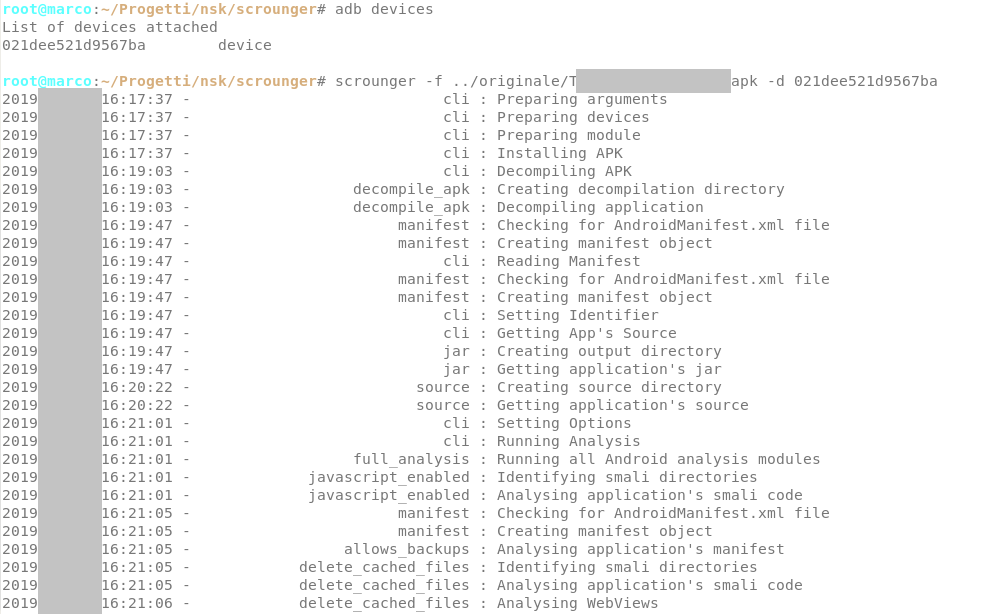
\includegraphics[width=.85\textwidth]{/scrounger/startCensBN}} 
	\caption{Full analysys.}
	\label{fig:start}
\end{figure}

Una volta terminata la scansione, i risultati vengono visualizzati a schermo e viene generato un report in formato \emph{JSON}.